\section{Path tracing naïf}

\subsection{Rappel de l'estimateur de Monte Carlo et de l'équation de rendu}

le Path Tracing est une technique de rendu d'image 3D visant à simuler de manière réaliste les rayons lumineux dans une scène. Pour se faire, nous nous sommes basé sur l'équation de rendu, théorisée par James Kajiya en 1986\footnote{Kay T. L., Kajiya J. T., Ray Tracing Complex Scenes, SIGGRAPH 1986.}:

$$\boxed{L_{o}(x, \omega_o) = L_{e}(x, \omega_o) + \int_{\Omega}f(x, \omega_o, \omega_i) \, L_{i}(x, \omega_i) \, \cos\left(\theta_i\right) \, d_{\omega_i}}$$

avec: 
\begin{itemize}
\item[$\_$] $\overrightarrow{n}$ : La normale de la surface au point $x$.
\item[$\_$] $\Omega$ : L'hémisphère centré autour de la normale $\textbf{n}$.
\item[$\_$] $x$ : Le point de $\mathbb{R}^3$ d'intersection entre les rayons incidents et la surface de l'objet considéré.
\item[$\_$] $\overrightarrow{\omega_o}$ : Direction du rayon réfléchis dans $\Omega$ sur la surface au point $x$.
\item[$\_$] $\overrightarrow{\omega_i}$ : Directions des rayons incidents dans $\Omega$ sur la surface au point $x$.
\item[$\_$] $L_o$ : La radiance réfléchis sur la surface au point $x$ de direction $\overrightarrow{\omega_o}$.
\item[$\_$] $L_e$ : La radiance émise par la surface au point $x$ de direction $\overrightarrow{\omega_o}$.
\item[$\_$] $L_i$ : Les radiances des rayons incidents sur la surface au point $x$ de direction $\overrightarrow{\omega_i}$.
\item[$\_$] $f$ : Le BRDF qui représente la manière dont le matériaux reflète la lumière.
\end{itemize}
\vspace{5mm}

Cette équation n'étant pas résolvable de manière analytique. Pour se faire, nous utiliserons la méthode Monte Carlo. En effet, cette méthode est la seule méthode qui passe à l'échelle face à la dimension infinie de l'équation de rendu.\\
Cette méthode se traduit de la manière suivante:\\
Soit une fonction $g:\left\{\mathbb{R} \longmapsto \mathbb{R}\atop x\longrightarrow g(x)\right.$ et $I$ l'integrale de $g$ dans $\Omega$. $I$ peut s'exprimer de la manière suivante:
$$
I = \int_\Omega g(x) \, d_x \approx \frac{1}{N} \sum_k^N \frac{g(x_k)}{\text{pdf}(x_k)}
$$

où $x_k$ est la k-ème variable aléatoire, tirée avec la loi de probabilité de densité $\text{pdf}(x)$. La somme converge en O$\left(\frac{1}{\sqrt{N}}\right)$. \\

Ainsi, l'estimateur Monte Carlo de l'équation de rendu s'écrit :\\


$$L_{o}(x, \omega_o) = L_{e}(x, \omega_o) + \sum_k^N\frac{f(x, \omega_o, \omega_k) \, L_{i}(x, \omega_k)}{\text{pdf}(\omega_k)} \, \cos\left(\theta_i\right) \, d_{\omega_i}$$
où les directions $\vec\omega_k$ sont tirées selon $\text{pdf}(\omega)$. Or $L_{i}(x, \omega_i)$ est elle-même définie par la même équation de rendu au point d'intersection suivant. L'estimateur est donc récursif : évaluer $\L_o$ en un point nécessite d'évaluer $L_i$ au point suivant, et ainsi de suite.\\

Un chemin de longueur d est une séquence de points d'intersection $\left( x_0,...,x_d\right)$, où $x_0$ est la caméra, $x_k$ le point d'intersection avec la k-ème primitive du chemin et $x_d$ est la source de lumière. La contribution d'un chemin pour un échantillon sera donc pour un échantillonnage pondéré par le cosinus ($\text{pdf}(\vec\omega)=\vec\omega\bullet\vec n/\pi=\cos(\theta)/\pi$, avec $\vec n$ la normal sortante de l'objet intersecté au point d'intersection entre le rayon et cette dernière) et avec seulement des matériaux lambertiens ($f(x, \omega_o, \omega)=\text{albedo}/\pi$):

$$
C=L_e(x_d)\cdot\prod^{d-1}_{k=1}\frac{f(x, \omega_o, \omega_k)\cdot\cos(\theta_k)}{\text{pdf}(\omega_k)}=L_e(x_d)\cdot\prod^{d-1}_{k=1}\text{albedo}_k
$$


En pratique, on tire $N=1$ chemin par pixel à chaque samples, et on moyenne les contributions sur l'ensemble des samples pour faire converger l'estimateur. Cela nous donnera ainsi la couleur d'un pixel.\\



Complexité de la méthode par rayon : O(N) pour N primitives\\
Complexité de la méthode : O$(N\cdot P\cdot n)$ pour $N$ primitives, $P$ pixels et $n$ chemins par pixels \\
Convergence: lente en $1\over{\sqrt(n)}$


\subsection{Implémentation}

Les primitives sont rangés dans un tableau de la structure suivante:

\begin{lstlisting}[language=C]
typedef struct Primitive
{
    void *object;
    Vector position;
    Vector color;
    PRIM_TYPE type;
    material_t m_type;
    float albedo;
} Primitive;
\end{lstlisting}

Ainsi, pour un pixel, nous ferons l'algorithme suivant pour déterminer la contribution $C$ d'un chemin:
\begin{algorithm}
\caption{Algorithme de la contribution d"un chemin}
\begin{algorithmic}
\Require Rayon $r$, sc\`ene $S$, cam\'era $cam$, profondeur max $d_{\max}$
\Ensure Contribution $C$
\State Initialiser $T \gets (1,1,1)$
\State Initialiser $r_{actuel} \gets r$
\For d=(1,...,$d_{max}$)
\If{pas d'intersection de $r_{actuel}$ avec la sc\`ene}
  \State \Return couleur de fond de la sc\`ene
\EndIf
\If{l'objet est émissif}
    \State $C \gets intensite\cdot couleur\_objet\cdot T$
    \State \Return $L$
\EndIf
\State G\'en\'erer un rayon réfléchi $r_{new}$ dans l'h\'emisph\`ere

\State $T \gets T\cdot albedo \cdot couleur\_objet$ 
\State$r_{actuel} \gets r_{new}$
\EndFor
\State \Return $C$
\end{algorithmic}
\end{algorithm}

\subsection{Premières analyses}

Le flame graphe (cf Figure 1.1) nous permet de remarquer les différents points chauds:


\begin{figure}[H]
\centering
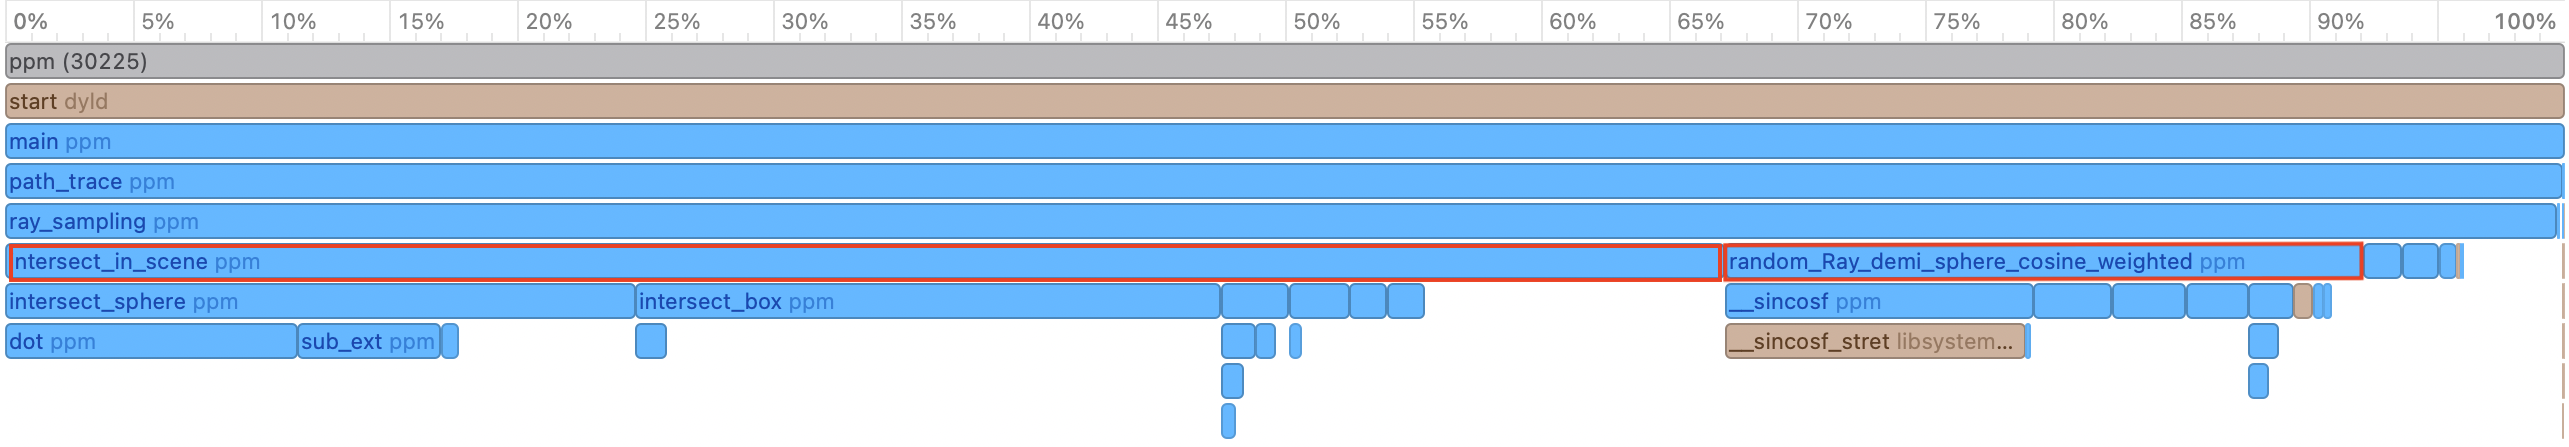
\includegraphics[scale=0.4]{include/flame_graph.png}
\caption{Flame Graphe du path tracer naïf avec Instruments.app. On constate 2 points chauds: \textit{intersect\_in\_scene} et \textit{random\_Ray\_demi\_sphere\_cosine\_weighted} (encadrés en rouge)}
\end{figure}


Ainsi, nous allons focaliser nos amélioration sur la diminution des calculs d'intersections ainsi que du nombre de rayons créés par chemin. 
Pour ce projet, nous avons sélectionné plusieurs améliorations structurelles afin de limiter les calculs d'intersections ainsi que de la création de rayons. Les optimisations que nous avons utilisé sont les suivantes:

\begin{itemize}
	\item[$\bullet$] Roulette russe
	\item[$\bullet$] Arbre BVH
	\item[$\bullet$] Clustering K-Means
	\item[$\bullet$] Bidirectional Path Tracing
\end{itemize}

